--
timeline vs outer - loop interchanged after ...
- loop interchangeability
: Loop interchange is the concept of reordering the dimensions of a loop. And
is ... MISSING
By inlining the \textbf{value} function [show code] we can split the loop and
perform the loop interchange between the two outer loops.
We know that this transformation is safe in this case because MISSING

\subsection{Loopinterchange}
If we inline the function \textbf{value} into the main loop we get what Figure
\ref{fig:inline_value} shows.

\begin{figure}[!ht]
	\centering
		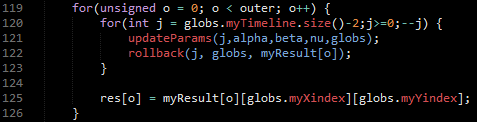
\includegraphics[scale=1]{input/figures/inline_value.png}
		\caption{The main loop where \textbf{value} is inlined.\label{fig:inline_value}}
\end{figure}

We can see that we can perform loop distribution on the inner loop and the
write to \emph{res}. By doing so, we are now able to loopinterchange the two
outer loops calling \textbf{updateParams} and \textbf{rollback} as we can see in
Figure \ref{fig:main_loopinterchange}.

\begin{figure}[!ht]
	\centering
		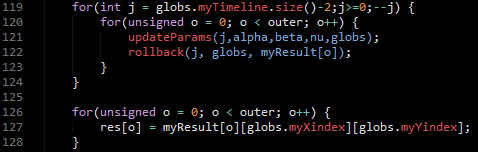
\includegraphics[scale=1]{input/figures/main_loopinterchange.png}
		\caption{The main loop where a loopinterchange has been performed.\label{fig:main_loopinterchange}}
\end{figure}

Our loopinterchange is safe \textbf{why?}.